AFGMiner generates and tests candidate patterns with increasing number of edges, then extends those patterns considered heavyweight. It generates candidate patterns of $k$ edges, starting with $k = 0$ (patterns composed of a single node and no edges), and searches for occurrences of such patterns in the dataset by using a sub-graph isomorphism detection algorithm, modified to take attributes into consideration~\cite{GomesMSc12}. The prototype implementation of AFGMiner adapts VF2~\cite{Cordella}, an algorithm that is faster than alternatives for graphs that are relatively regular, have a large number of nodes and whose nodes have small valency~\cite{Foggia}, such as the ones found in the case study. Each occurrence found has its node weight and edge weight support values computed, and, when no more occurrences of a pattern are present in the dataset, the support value for the pattern itself is computed by aggregating the support values of its occurrences. If the support value for the pattern is higher than an user-defined threshold, the pattern is heavyweight. It is then output to the user and later extended into candidate patterns with an additional edge, a process called \emph{edge-by-edge pattern extension}. If the pattern is not heavyweight, it is discarded. Edge-by-edge pattern extension works by adding to a pattern either: (i) an edge that connects two of its nodes; (ii) or an edge that connects one of its nodes to a new node called the \emph{extension node}. A pattern that generates other patterns by extension is called a \emph{parent pattern}, while the generated patterns are \emph{child patterns}.

\subsection{Canonical Labeling}
Two different patterns, when extended, may generate child patterns that are isomorphic. Thus, redundancy should be detected using the well-known concept of \emph{canonical labelling}~\cite{gSpan}. The idea is to map each sub-graph pattern to an identifier string called \emph{DFS Code} after labelling its nodes and edges. DFS Codes can then be lexically ordered in such a way that, if two sub-graphs are isomorphic to each other, they provably have the same minimum DFS Code. The rules that define how to sort DFS Codes depend on the types of graphs being mined~\cite{GomesMSc12}.

\subsection{Support Value Policy}
AFGMiner adopts an \emph{anti-monotonic} support-value policy to enable the pruning of its search space. Under this policy, the support value of a pattern is always lower than or equal to the support value of any of its ancestor patterns. Therefore, if a pattern is not heavyweight, none of its descendants can be heavyweight. Therefore, all patterns that do not meet a minimum support criteria can be discarded. The support-value policy works as follows. For each occurrence $g$ of a pattern $p$, two values are calculated: $S_n(g)$, the weight of the attribute with minimum weight amongst all attributes associated with nodes of $g$; and $S_e(g)$, the minimum edge weight amongst all edges of $g$. The $S_n(g)$ of all occurrences of $p$ found in $DS$ are then added up, resulting in $S_n(p)$, the node-weight support of $p$. The $S_e(g)$ of all occurrences of $p$ found in $DS$ are also added up, resulting in $S_e(p)$, the edge-weight support of $p$. The support value for $p$ is $S_m(p)$, the maximum between $S_n(p)$ and $S_e(p)$. $S_m(p)$ is compared against the support threshold to decide whether $p$ is a heavyweight pattern. The support-value policy selected for AFGMiner is anti-monotonic because only the minimum edge weight and the minimum node attribute weight of each occurrence are used in the computation.

\subsection{Generation of Candidate Patterns}
AFGMiner mines for candidate patterns with an increasing number of attributes in their single node (in the case of 0-edge patterns) or in their extension node (in the case of $k$-edge patterns with $k > 0$), starting with a single attribute, and then combining attributes such that an attribute set is used to generate a pattern only if all of its sub-sets generated heavyweight patterns. This process is called \emph{attribute-set growth}. A set of patterns that have the same number of edges is called a \emph{generation}. Patterns of a certain generation are only created and mined after all the heavyweight patterns of the previous generation have been found. This is important because it allows the algorithm to use only the $A_k$ set of distinct attributes present in the $(k - 1)$-th generation to compose the patterns of the $k$-th generation, thus restricting the number of candidate patterns produced.

%\begin{figure}[h!]
%\centering
 %   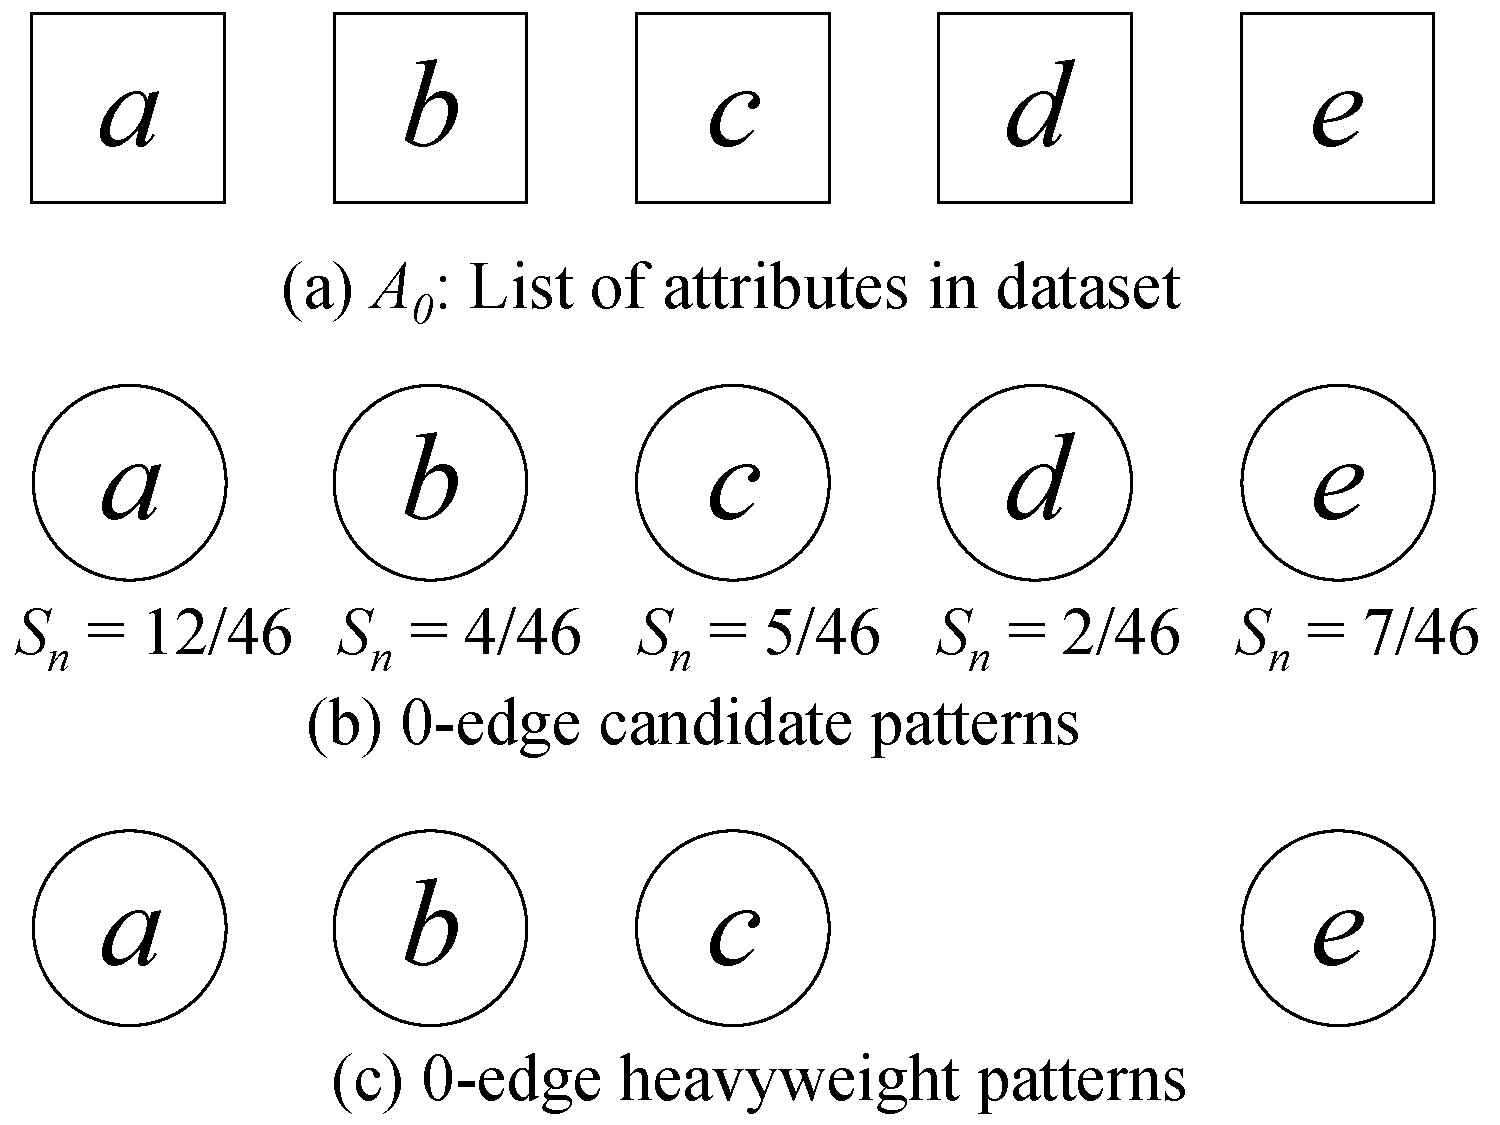
\includegraphics[scale=0.15]{figures/example_0-edge.pdf}
   % \caption{0-edge candidate patterns.}
    %\label{fig:example_0-edge}  
%\end{figure}

%\begin{figure}[h!]
%\centering
   % 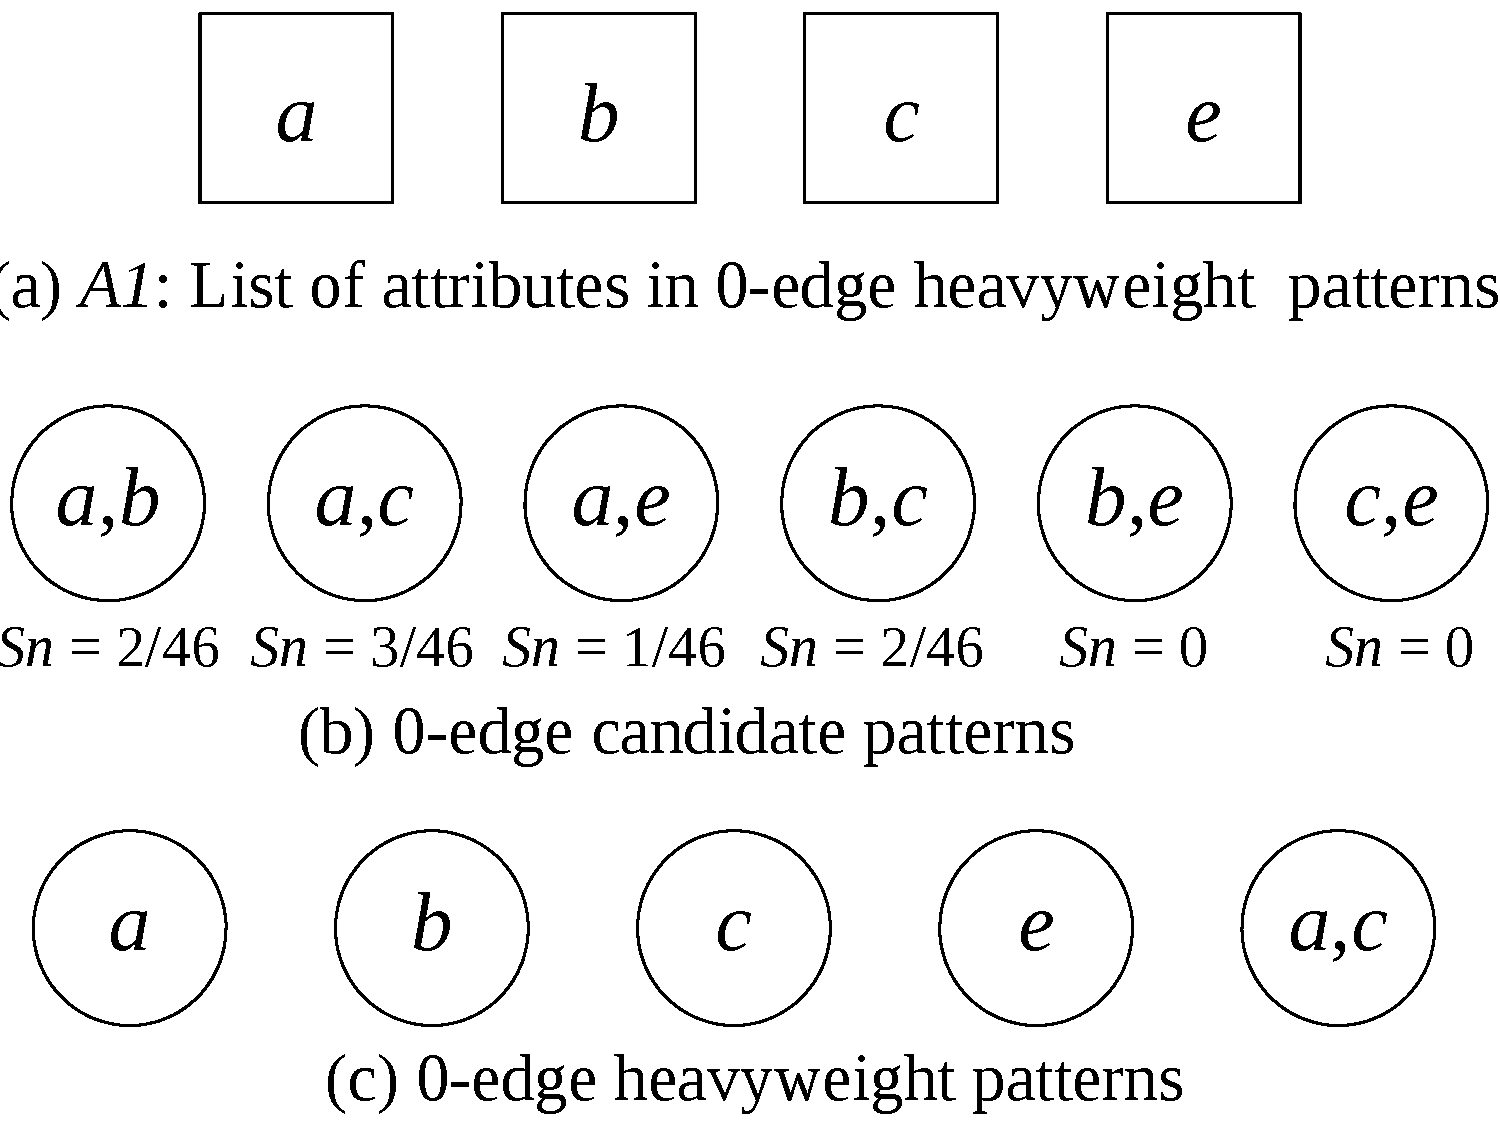
\includegraphics[scale=0.15]{figures/example_0-edge_2-attribute.pdf}
    %\caption{Attribute-set growth for 0-edge candidate patterns.}
    %\label{fig:example_0-edge_2-attribute}  
%\end{figure}

%\begin{figure}[h!]
%\centering
   % 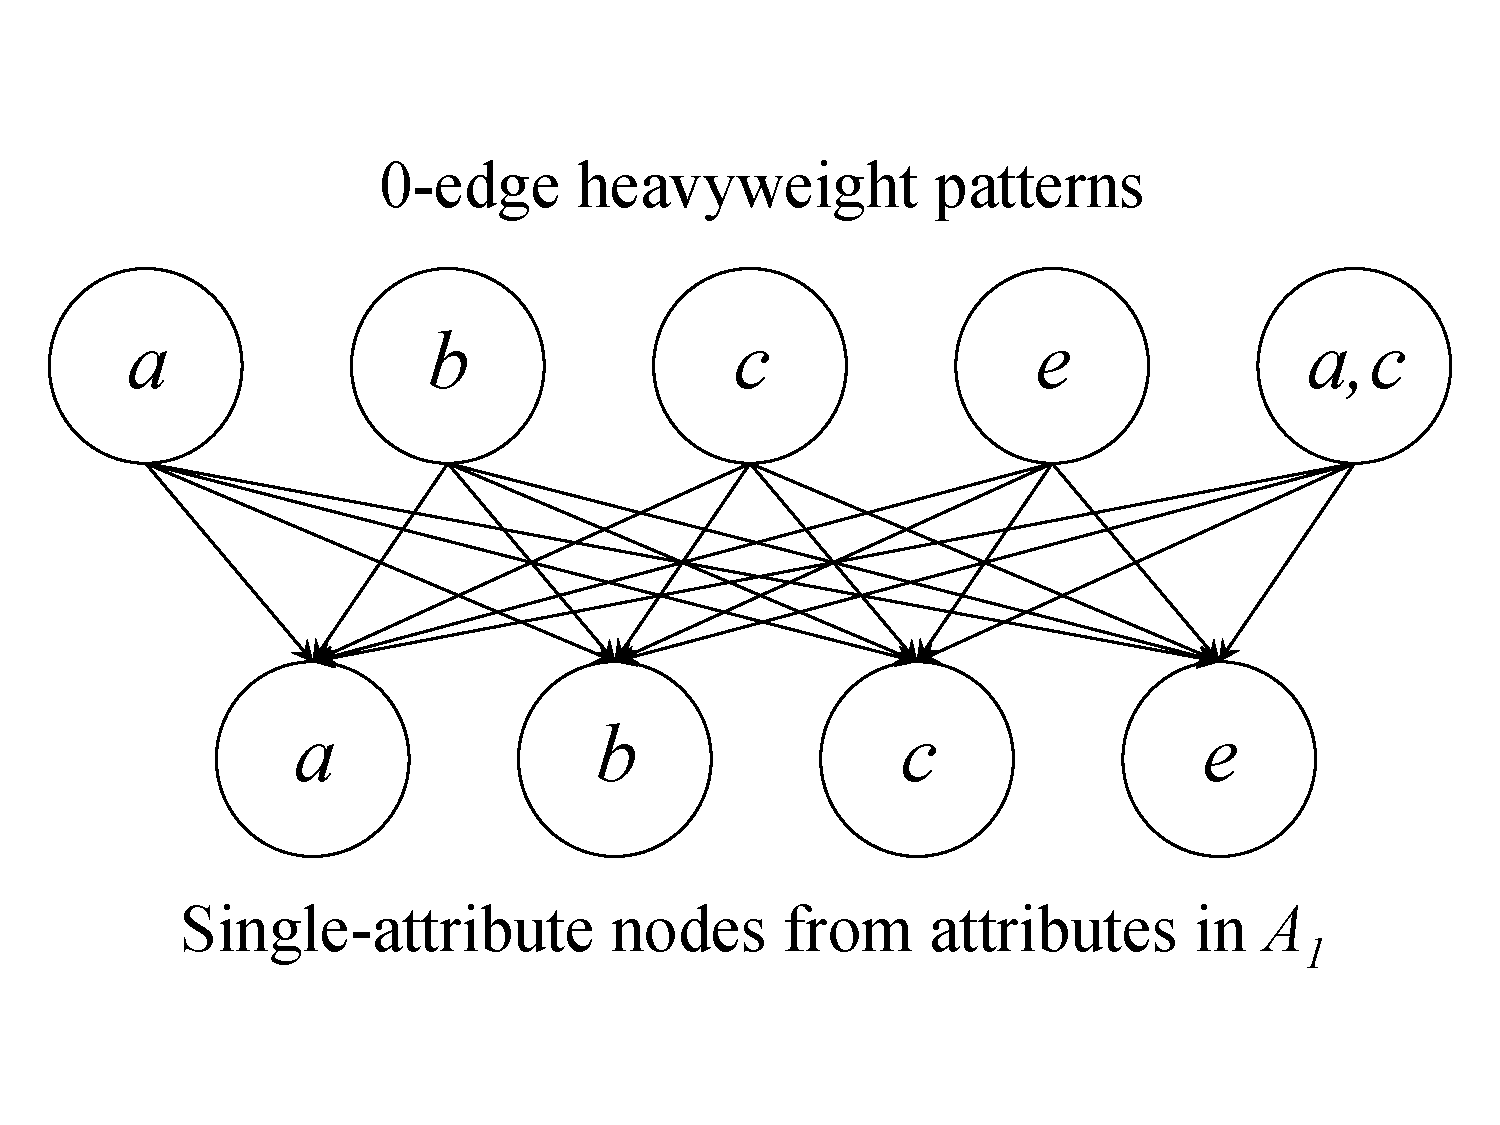
\includegraphics[scale=0.15]{figures/example_1-edge.pdf}
    %\caption{1-edge candidate patterns.}
    %\label{fig:example_1-edge}  
%\end{figure}

%\begin{figure}[h!]
%\centering
  %  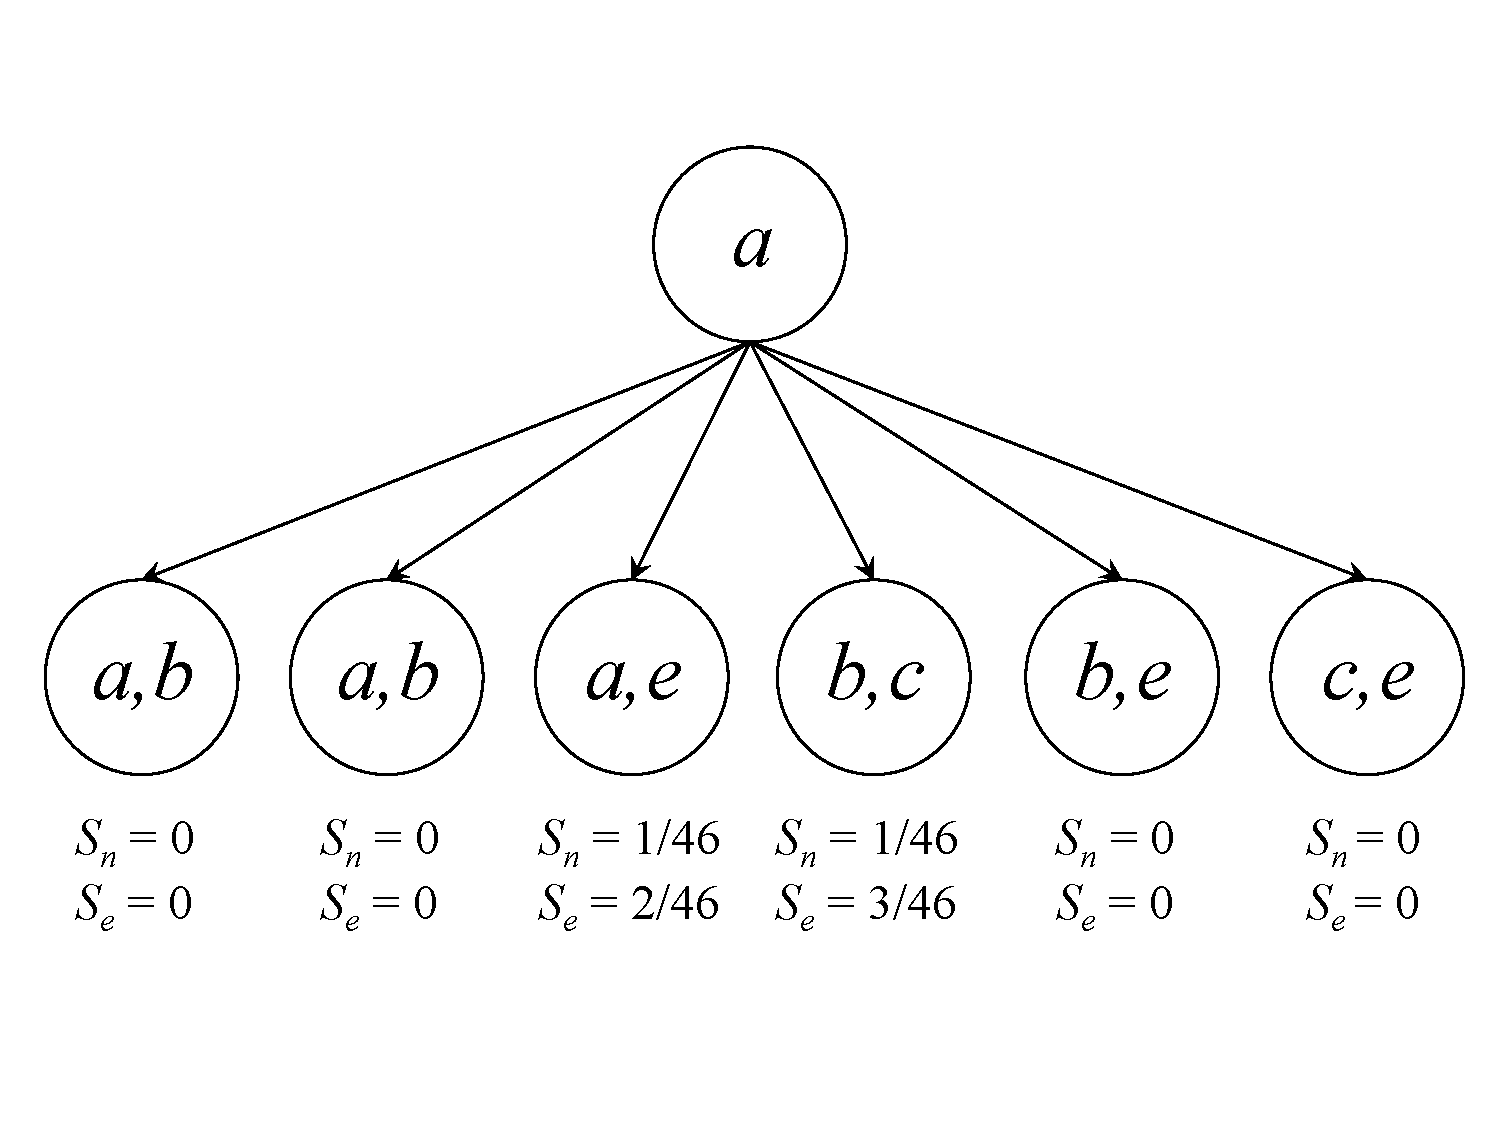
\includegraphics[scale=0.15]{figures/example_1-edge_2-attribute.pdf}
   % \caption{Attribute-set growth for 1-edge candidate pattern node $a$ $\rightarrow$ $a$. }
    %\label{fig:example_1-edge_2-attribute}  
%\end{figure}

%\begin{figure}[h!]
%\centering
 %   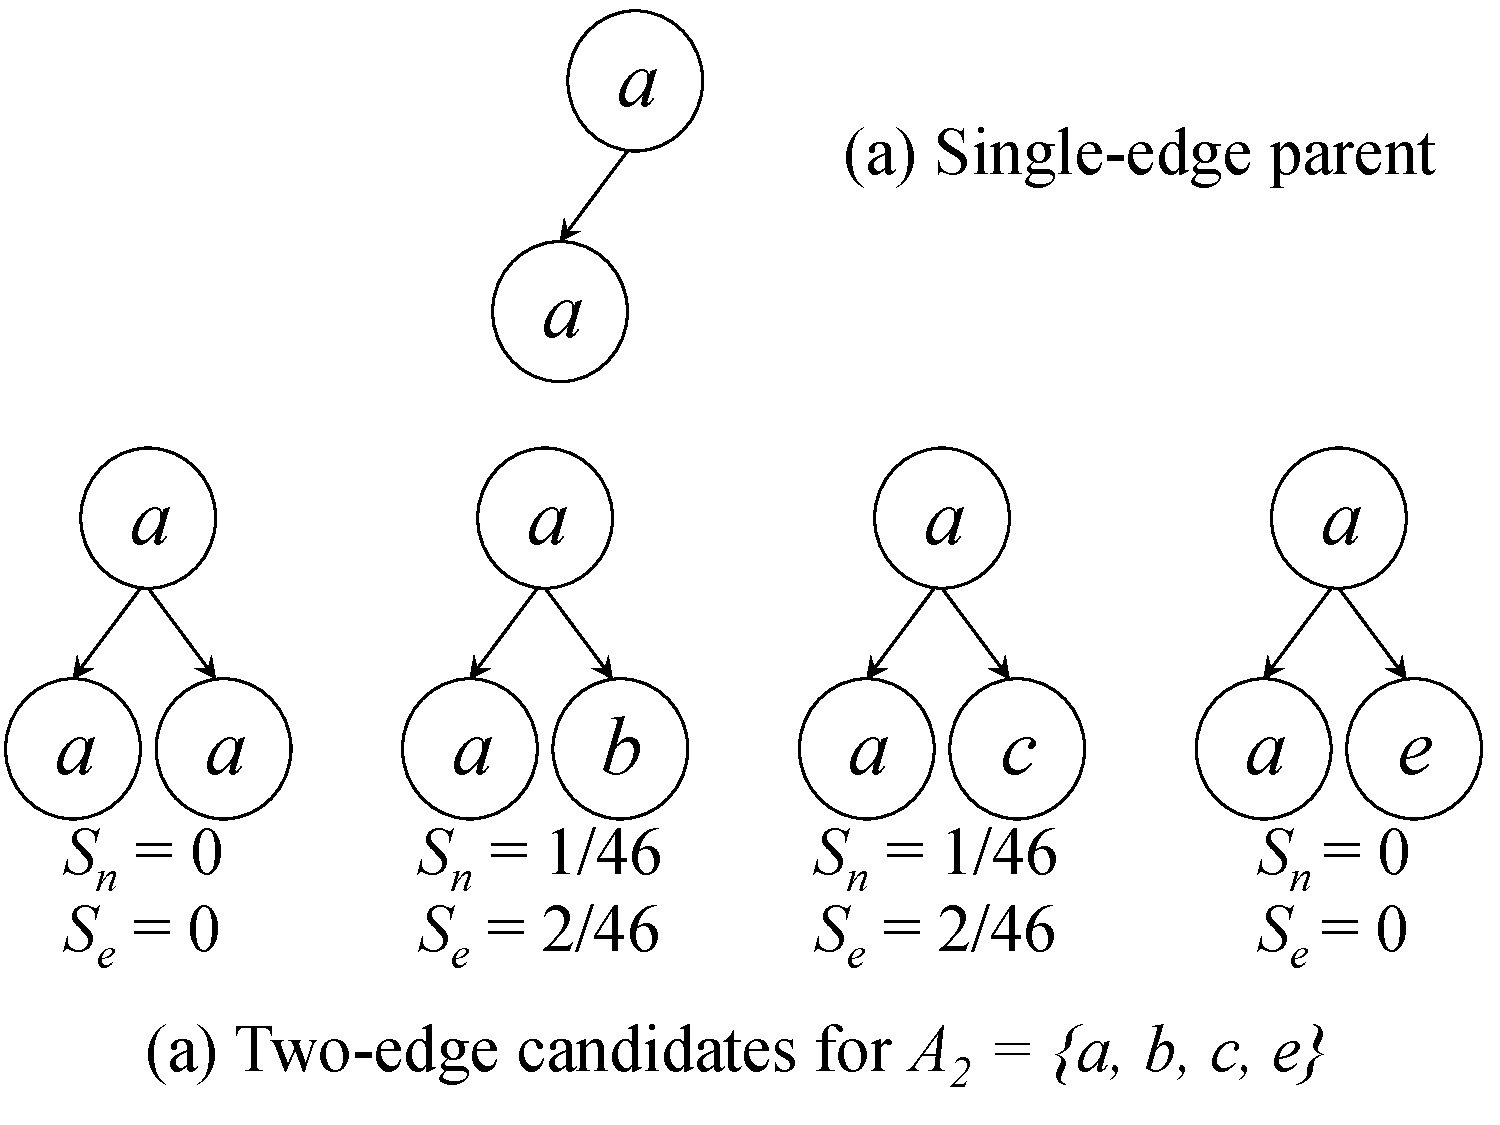
\includegraphics[scale=0.15]{figures/example_2-edge.pdf}
  %  \caption{2-edge candidate patterns.}
   % \label{fig:example_2-edge}  
%\end{figure}

